%
% 	OPEN OBJECTS AND REWRITING
%	open object
%	v1
%

% comment out when compiling 
%%
%	REWRITING OPEN GRAPHS
%	preamble
%	v1

%  packages

\usepackage{amsfonts, amsthm, amssymb, amsmath, stmaryrd, etoolbox}
\usepackage{mathtools}
\usepackage{graphicx,caption,subcaption}
\usepackage{todonotes}
\usepackage{xcolor}
\usepackage{url}
\usepackage[inline]{enumitem}
	\setlist{itemsep=0em, topsep=0em, parsep=0em}
	\setlist[enumerate]{label=(\alph*)}
\usepackage[]{hyperref}
	\definecolor{hyperrefcolor}{rgb}{0,0,0.7}
	\hypersetup{colorlinks,linkcolor={hyperrefcolor},citecolor={hyperrefcolor},urlcolor={hyperrefcolor}}
\usepackage{tikz}
	\usetikzlibrary{matrix,arrows,shapes,decorations.markings,decorations.pathreplacing}
\usepackage[numbers]{natbib}
\usepackage{doi}

%
% commands
%

\newcommand{\RR}{\mathbb{R}}
\newcommand{\ZZ}{\mathbb{Z}}
\newcommand{\NN}{\mathbb{N}}
\newcommand{\QQ}{\mathbb{Q}}
\newcommand{\CC}{\mathbb{C}}
\newcommand{\DD}{\mathbb{D}}
\newcommand{\MM}{\mathbb{M}}
\renewcommand{\epsilon}{\varepsilon}

\newcommand{\defn}[1]{\textbf{#1}}
\newcommand{\op}[1]{\operatorname{#1}}
\newcommand{\cat}[1]{\mathbf{#1}}
\newcommand{\dblcat}[1]{\mathbb{#1}}
\renewcommand{\t}[1]{\text{#1}}

\newcommand{\from}{\colon}
\newcommand{\xto}[1]{\xrightarrow{#1}}
\newcommand{\sm}{\smallsetminus}
\newcommand{\tospan}{\xrightarrow{\mathit{sp}}}
\newcommand{\tocospan}{\xrightarrow{\mathit{csp}}}
\newcommand{\diagram}[1]{\raisebox{-0.5\height}{\includegraphics{#1}}}

\newcommand{\bispmap}[1]{\mathbf{Sp(#1)}}
\newcommand{\dblspmap}[1]{\mathbb{S}\mathbf{p(#1)}}
\newcommand{\bicspmap}[1]{\mathbf{Csp(#1)}}
\newcommand{\dblcspmap}[1]{\mathbb{C}\mathbf{sp(#1)}}
\newcommand{\bispsp}[1]{\mathbf{Sp(Sp(#1))}}
\newcommand{\dblspsp}[1]{\mathbb{S}\mathbf{p(Sp(#1))}}
\newcommand{\bicspcsp}[1]{\mathbf{Csp(Csp(#1))}}
\newcommand{\dblcspcsp}[1]{\mathbb{C}\mathbf{sp(Csp(#1))}}
\newcommand{\bimonspcsp}[1]{\mathbf{MonicSp(Csp(#1))}}
\newcommand{\dblmonspcsp}[1]{\mathbb{M}\mathbf{onicSp(Csp(#1))}}
\newcommand{\biepiccspsp}[1]{\mathbf{EpicCsp(Sp(#1))}}
\newcommand{\dblepiccspsp}[1]{\mathbb{E}\mathbf{picCsp(Sp(#1))}}
\newcommand{\spcsp}[1]{\mathbf{Sp(Csp(#1))}}
\newcommand{\dblspcsp}[1]{\mathbb{S}\mathbf{p(Csp(#1))}}

\newcommand{\LspanD}{ L \t{-} \operatorname{Span} ( \mathbf{D} ) }
\newcommand{\LopenD}{ L \t{-} \operatorname{Open} }
\newcommand{\LrewriteD}{ L \t{-} \operatorname{Rewrite} }

%
% math operators
%

\DeclareMathOperator{\Hom}{Hom}
\DeclareMathOperator{\id}{id}
\DeclareMathOperator{\ob}{Ob}
\DeclareMathOperator{\arr}{arr}
\DeclareMathOperator{\im}{im}
\DeclareMathOperator{\Aut}{Aut}
\DeclareMathOperator{\Bij}{Bij}
\DeclareMathOperator{\Sub}{Sub}
\DeclareMathOperator{\colim}{colim}

%
% envirnments and counters
%

\newtheorem{thm}{Theorem}[section]
\newtheorem{lem}[thm]{Lemma}
\newtheorem{prop}[thm]{Proposition}
\newtheorem{cor}[thm]{Corollary}

\theoremstyle{remark}
	\newtheorem{remark}[thm]{Remark}
	\newtheorem{notation}[thm]{Notation}

\theoremstyle{definition}
	\newtheorem{ex}[thm]{Example} 
	\newtheorem{df}[thm]{Definition}

% \setcounter{tocdepth}{1} % Sets depth for table of contents. 

%
% tikz types
%

\tikzset{->-/.style={decoration={%
			markings,
			mark=at position .5 with {\arrow{>}}},postaction={decorate}}
}
\tikzset{->-pos/.style={decoration={%
			markings,
			mark=at position #1 with {\arrow{>}}},postaction={decorate}}
}
\tikzset{->-/.style={decoration={%
			markings,
			mark=at position .5 with {\arrow{>}}},postaction={decorate}}
}
\tikzset{->-pos/.style={decoration={%
			markings,
			mark=at position #1 with {\arrow{>}}},postaction={decorate}}
}
 % input preamble
%\bibliography{3--RewriteOpenGraphs--Bibliography}	

%%%%%%%%%%%%%%%%%%%%%
\section{A motivating example}
\label{sec:MotivatingExample}
%%%%%%%%%%%%%%%%%%%%%

\todo{
	intro to section
}

\todo{
	rewrite this section.
	its exactly from 
	zx-calc paper
}
Conceptually, open graphs 
are quite simple.  
Take a directed graph 
and declare some of the nodes 
to be inputs and 
others to be outputs, 
for example
\begin{equation}
\label{ex--OpenGraph1}
	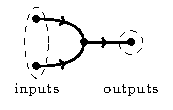
\includegraphics{InclGrphx--Example--OpenGraph1}
\end{equation}

Given open graphs $G$ and $G'$,
if the set of inputs in $G$
and the set of outputs in $G'$
have the same cardinality,
we can glue them together
along a bijection.
This gives a way 
to turn a pair of 
compatible open graphs
into a single open graph.  
For instance, 
to the above open graph, 
we can connect 
\begin{equation}
\label{ex--OpenGraph2}
	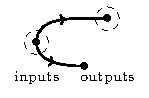
\includegraphics{InclGrphx--Example--OpenGraph2}
\end{equation}
to form
\begin{equation}
	\label{ex--OpenGraph3}
	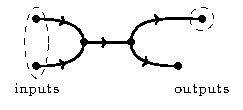
\includegraphics{InclGrphx--Example--OpenGraph3}
\end{equation}
We make this precise with
cospans and pushouts.

\todo{
	past considerations of open graphs
}

Consider the functor
\begin{equation}
\label{eq--FunctorN}
	N \colon \mathbf{FinSet} \to \mathbf{Graph},
\end{equation}
defined by the letting 
$N(X)$ be the edgeless graph 
with nodes $X$.  

\begin{df} % open graphs
\label{df--OpenGraph}
	An \emph{open graph} is then 
	a cospan in the category 
	$\mathbf{Graph}$ 
	of the form 
	$N(X) \to G \gets N(Y)$ 
	for sets $X$ and $Y$.
	Given another open graph
	$N(X') \to G' \gets N(Y')$, 
	a morphism between them
	is a triple $(f,g,h)$ so that
	the diagram
	\[
		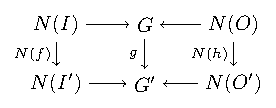
\includegraphics{InclGrphx--Diagram--OpenGraphMap}
	\]
	commutes.
	Open graphs and their morphisms
	form a category $\cat{OpenGraph}$.	
\end{df}

Isomorphisms of open graphs
play an important role 
for the theory developed in this paper.  
Of particular note are the \defn{globular morphisms},
which are those where 
$f$ and $h$ are identities.  

How does a cospan outfit a graph
with inputs and outputs?
The left leg $N(X)$ of the cospan 
selects the \emph{inputs} and 
the right leg $N(Y)$ the \emph{outputs}.  
We will refer to the union
of the inputs and outputs as the
\emph{interface} of an open graph.
The addition of an interface allows us to 
`glue' certain open graphs together
to produce another open graph.
Indeed, suppose we have open graphs 
\[
	N ( X ) \to G \gets N ( Y )
	\t{ and }
	N ( Y ) \to H \gets N ( Z ).
\]
Then we can concatenate the cospans 
\[
	N(X) \to G \gets N(Y) \to H \gets N(Z). 
\] 
and obtain another open graph
by pushing out over 
$G \gets N(Y) \to G'$ to get 
\[
	N(X) \to G +_{ N ( Y ) } H \gets N(Z).
\] 

To illustrate this, 
realize the open graph in \eqref{ex--OpenGraph1}
as the cospan of graphs
\begin{equation}
\label{ex--OpenGraphCospan1}
	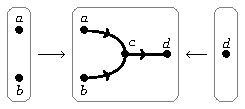
\includegraphics{InclGrphx--Example--OpenGraphCospan1}
\end{equation}
Similarly, we realize \eqref{ex--OpenGraph2} as 
\[
	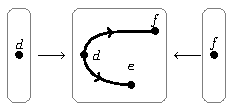
\includegraphics{InclGrphx--Example--OpenGraphCospan2}
\]
Now, pushout over
the middle span in the concatenated
cospans
\[
	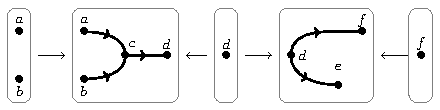
\includegraphics{InclGrphx--Example--OpenGraphCospan3}
\]
The result is
\[
	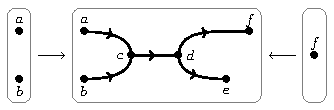
\includegraphics{InclGrphx--Example--OpenGraphCospan4}
\]
which realizes 
\eqref{ex--OpenGraph3} 
as a cospan.

In fact, this manner of 
connecting open graphs together
serves as composition 
in a category whose objects are 
those in the image of the functor $N$
(see definition \ref{def:OpenGraph})
and whose morphisms are open graphs
up to globular isomorphism.  
But this is just the first layer 
of a richer structure!
In a sense, we can endow
the hom-spaces of this category
with the structure of the category
$\cat{OpenGraph}$ mentioned above,
giving a bicategory consisting of
edgeless graphs, 
open graphs, and
globular morphisms of open graphs.
While this bicategory is interesting
itself, it is too limiting 
for our intended uses.  
Indeed, we are interested in
an upgraded version
where the 2-cells are
rewrites of open graphs.
Indeed, there is a bicategory 
$\cat{Rewrite}$ introduced by the author
\citep{Cicala_SpansCospans}
consisting of edgeless graphs,
open graphs, and 
monic-legged spans of open graphs. 
It was even shown to be 
symmetric monoidal and compact closed
\citep{CicalaCourser_BicatSpansCospan}.
The motivation for naming $\cat{Rewrite}$
as we did is that 
monic-legged spans of open graphs
as 2-cells are intended to
capture the idea of 
double pushout graph rewriting.  
This paper seeks to explore further
the rewriting of open graphs.  
We even revisit $\cat{Rewrite}$
while applying open graphs
to categorify $\cat{2Cob}$
in Section 
\todo{reference application section here}
But first, we develop the
rewriting theory of open graphs.

\todo{show cat of oGraphs is topos so adhsv}






